\begin{center}
    {\LARGE \textbf{2012物理化学}} \\[2ex]
    {\large 时量180分钟 \quad 满分150分}
\end{center}

\vspace{0.5cm}
\noindent\textbf{注意事项:}
\begin{enumerate}[label=\arabic*., parsep=0pt, itemsep=0pt]
    \item 答题前,考生先将自己的姓名、学号、考场号、座位号填写在答题卡上,将条形码准确粘贴在考生信息条形码粘贴区。
    \item 考试结束后,将本试卷与答题纸一并收回。
    \item 回答各个问题时,将答案写在答题纸上,写在本试卷上无效。
\end{enumerate}

\vspace{0.5cm}
\noindent\textbf{一、选择题(30 pts.)}

\begin{enumerate}[label=\arabic*., itemsep=1.5ex]
    \item 气体$\ce{CO}$和$\ce{N2}$有相近的转动惯量和相对分子摩尔质量,在相同温度和压力时,两者平动和转动熵的大小为
    \begin{tasks}(1)
        \task $S_{\text{t,m}}(\ce{CO})=S_{\text{t,m}}(\ce{N2})$,\quad $S_{\text{r,m}}(\ce{CO})>S_{\text{r,m}}(\ce{N2})$
        \task $S_{\text{t,m}}(\ce{CO})>S_{\text{t,m}}(\ce{N2})$,\quad $S_{\text{r,m}}(\ce{CO})>S_{\text{r,m}}(\ce{N2})$
        \task $S_{\text{t,m}}(\ce{CO})=S_{\text{t,m}}(\ce{N2})$,\quad $S_{\text{r,m}}(\ce{CO})<S_{\text{r,m}}(\ce{N2})$
        \task $S_{\text{t,m}}(\ce{CO})=S_{\text{t,m}}(\ce{N2})$,\quad $S_{\text{r,m}}(\ce{CO})=S_{\text{r,m}}(\ce{N2})$
    \end{tasks}
    \item (1)$\ce{NaOH}$溶解于水
    (2)水溶液中,$\ce{Ag^+ + 2NH3(g) -> [Ag(NH3)2]^+}$
    (3)$\ce{HCl}$气体溶于水,生成盐酸
    (4)$\ce{2KClO3(s) -> 2KCl(s) + 3O2(g)}$
    (5)$\ce{NH4Cl(s) -> NH3(g) + HCl(g)}$
    上述各体系在等温等压过程中熵值减少的是
    \begin{tasks}(4)
        \task (2),(3)
        \task (1),(4)
        \task (4),(5)
        \task (1),(2)
    \end{tasks}
    \item 已知有下列一组公式可用于理想气体绝热过程功的计算:
    \begin{enumerate}[label=(\arabic*), itemsep=1ex]
        \item $W=C_V(T_1-T_2)$
        \item $[1/(\gamma-1)](p_1V_1-p_2V_2)$
        \item $[p_1V_1/(\gamma-1)][1-(V_1/V_2)^{\gamma-1}]$
        \item $[p_1V_1/(\gamma-1)][1-(p_2/p_1)^{(1-\gamma)/\gamma}]$
        \item $[p_1V_1/(\gamma-1)][1-(p_2V_2/p_1V_1)]$
        \item $[R/(\gamma-1)](T_1-T_2)$
    \end{enumerate}
    但这些公式只适于绝热可逆过程的是
    \begin{tasks}(4)
        \task (1),(2)
        \task (3),(4)
        \task (5),(6)
        \task (4),(5)
    \end{tasks}
    \item 若已知某溶液中物质$\ce{B}$的偏摩尔混合Gibbs自由能为$-889.62\ \mathrm{J\cdot mol^{-1}}$,温度为$300\ \mathrm{K}$,
    
    则$\ce{B}$的活度$a_x(\ce{B})$为
    \begin{tasks}(4)
        \task $0.65$
        \task $0.7$
        \task $0.8$
        \task $0.56$
    \end{tasks}
    \item 电导测定应用广泛,但下列问题中哪个是不能用电导测定来解决的?
    \begin{tasks}(2)
        \task 求难溶盐的溶解度
        \task 求弱电解质的解离度
        \task 求平均活度系数
        \task 测电解质溶液的浓度
    \end{tasks}
    \item $p^\ominus$和$298\ \mathrm{K}$下,把$\ce{Pb}$和$\ce{Cu(Ac)2}$溶液发生的反应安排为电池,当获得可逆电功为$91.84\ \mathrm{kJ}$
    
    时,电池同时吸热$213.6\ \mathrm{kJ}$,因此该过程有
    \begin{tasks}(2)
        \task $\Delta_\mathrm{r}U>0$,$\Delta_\mathrm{r}S>0$
        \task $\Delta_\mathrm{r}U<0$,$\Delta_\mathrm{r}S>0$
        \task $\Delta_\mathrm{r}U>0$,$\Delta_\mathrm{r}S<0$
        \task $\Delta_\mathrm{r}U<0$,$\Delta_\mathrm{r}S<0$
    \end{tasks}
    \item 苯在一个刚性的绝热容器中燃烧,
    \[
    \ce{C6H6(l) + (15/2)O2(g) <=> 6CO2 + 3H2O(g)}
    \]
    \begin{tasks}(2)
        \task $\Delta U=0$,\quad $\Delta H<0$,\quad $Q=0$
        \task $\Delta U=0$,\quad $\Delta H>0$,\quad $W=0$
        \task $\Delta U=0$,\quad $\Delta H=0$,\quad $Q=0$
        \task $\Delta U\neq0$,\quad $\Delta H\neq0$,\quad $Q=0$
    \end{tasks}
    \item 浓度为$1.0\ \mathrm{mol\cdot dm^{-3}}$的强电解质溶液,它的摩尔电导率数值近似于
    \begin{tasks}(2)
        \task 与电导率相等
        \task 是电导率的$10^3$倍
        \task 是电导率的$10^{-3}$倍
        \task 是电导率的$10^2$倍
    \end{tasks}
    \item 已知$25^\circ\mathrm{C}$时,电极反应$\displaystyle \frac{1}{2}\ce{O2 + H2O + 2e^- -> 2OH^-}$的标准电极电势为$\varphi_1^\ominus=0.401\ \mathrm{V}$,
    
    则$25^\circ\mathrm{C}$时,电极反应$\displaystyle \frac{1}{2}\ce{O2 + 2H^+ + 2e^- -> H2O}$的标准电极电势$\varphi_2^\ominus$为(设$K_\mathrm{w}=1\times10^{-14}$)
    \begin{tasks}(4)
        \task $-0.427\ \mathrm{V}$
        \task $0.401\ \mathrm{V}$
        \task $0.828\ \mathrm{V}$
        \task $1.229\ \mathrm{V}$
    \end{tasks}
    \item 在$298\ \mathrm{K}$下,将液体水分散成小液滴,其热力学能
    \begin{tasks}(4)
        \task 增加
        \task 降低
        \task 不变
        \task 无法判定
    \end{tasks}
    \item 当溶液中溶质浓度采用不同浓标时,下列说法中哪一个是正确的
    \begin{tasks}(2)
        \task 溶质的活度相同
        \task 溶质的活度系数相同
        \task 溶质的标准化学势相同
        \task 溶质的化学势相同
    \end{tasks}
    \item 当一反应物的初始浓度为$0.04\ \mathrm{mol\cdot dm^{-3}}$时,反应的半衰期为$360\ \mathrm{s}$,
    
    初始浓度为$0.024\ \mathrm{mol\cdot dm^{-3}}$时,半衰期为$600\ \mathrm{s}$,此反应为
    \begin{tasks}(4)
        \task $0$级反应
        \task $1.5$级反应
        \task $2$级反应
        \task $1$级反应
    \end{tasks}
    \item 在浓度为$c_1$的$\ce{HCl}$与浓度$c_2$的$\ce{BaCl2}$混合溶液中,离子迁移数可表示成
    \begin{tasks}(1)
        \task $\lambda_\mathrm{m}(\ce{H^+})/[\lambda_\mathrm{m}(\ce{H^+}) + \lambda_\mathrm{m}(\ce{Ba^{2+}}) + 2\lambda_\mathrm{m}(\ce{Cl^-})]$
        \task $c_1\lambda_\mathrm{m}(\ce{H^+})/[c_1\lambda_\mathrm{m}(\ce{H^+}) + 2c_2\lambda_\mathrm{m}(1/2\ce{Ba^{2+}}) + (c_1+2c_2)\lambda_\mathrm{m}(\ce{Cl^-})]$
        \task $c_1\lambda_\mathrm{m}(\ce{H^+})/[c_1\lambda_\mathrm{m}(\ce{H^+}) + c_2\lambda_\mathrm{m}(\ce{Ba^{2+}}) + \lambda_\mathrm{m}(\ce{Cl^-})]$
        \task $c_1\lambda_\mathrm{m}(\ce{H^+})/[c_1\lambda_\mathrm{m}(\ce{H^+}) + 2c_2\lambda_\mathrm{m}(\ce{Ba^{2+}}) + 2c_2\lambda_\mathrm{m}(\ce{Cl^-})]$
    \end{tasks}
    \item 根据理想稀溶液中溶质和溶剂的化学势公式:
    \[
    \mu_\mathrm{B} = \mu_\mathrm{B}^*(T,p) + RT\ln x_\mathrm{B},\quad \mu_\mathrm{A} = \mu_\mathrm{A}^*(T,p) + RT\ln x_\mathrm{A}
    \]
    下面叙述中不正确的是
    \begin{tasks}(1)
        \task $\mu_\mathrm{A}^*(T,p)$是纯溶剂在所处$T$、$p$时的化学势
        \task $\mu_\mathrm{B}^*(T,p)$是$x_\mathrm{B}=1$,且仍服从亨利定律的假想状态的化学势,而不是纯溶质的化学势
        \task 当溶质的浓度用不同方法(如$x_\mathrm{B}$,$m_\mathrm{B}$,$c_\mathrm{B}$)表示时,$\mu_\mathrm{B}^*(T,p)$不同,但$\mu_\mathrm{B}$不变
        \task $\mu_\mathrm{A}^*(T,p)$只与$T$,$p$及溶剂的性质有关,$\mu_\mathrm{B}^*(T,p)$只与$T$、$p$及溶质的性质有关
    \end{tasks}
    \item 在$288\ \mathrm{K}$时,$\ce{H2O(l)}$的饱和蒸气压为$1\ 702\ \mathrm{Pa}$,当$0.6\ \mathrm{mol}$的不挥发溶质$\ce{B}$
    
    溶于$0.540\ \mathrm{kg}\ \ce{H2O}$时,蒸气压下降$42\ \mathrm{Pa}$,溶液中$\ce{H2O}$的活度系数$\gamma_x$应该为
    \begin{tasks}(4)
        \task $0.980\ 4$
        \task $0.975\ 3$
        \task $1.005$
        \task $0.994\ 8$
    \end{tasks}
\end{enumerate}

\vspace{0.5cm}
\noindent\textbf{二、计算题(20 pts.)}

苯的正常凝固点和沸点分别是$278\ \mathrm{K}$和$353\ \mathrm{K}$,在$278\ \mathrm{K}$时$\Delta_{\mathrm{fus}}H_\mathrm{m}=-9.94\ \mathrm{kJ\cdot mol^{-1}}$,

$C_{p,\mathrm{m}}(\mathrm{l})$和$C_{p,\mathrm{m}}(\mathrm{s})$分别为$127$和$123\ \mathrm{J\cdot K^{-1}\cdot mol^{-1}}$。
\begin{enumerate}[label=(\alph*), itemsep=1ex]
    \item 在$353\ \mathrm{K}$、$p^\ominus$下的$1\mathrm{mol}$液态苯等温向真空变为$353\ \mathrm{K}$,$p^\ominus$的苯蒸气(设为理想气体)。
    \item 在$268\ \mathrm{K}$、$p^\ominus$下过冷液体苯凝固。
    \begin{enumerate}[label=(\arabic*), itemsep=1ex]
        \item 求算过程(a)的$Q$,$\Delta_{\mathrm{vap}}H_\mathrm{m}$,$\Delta_{\mathrm{vap}}S_\mathrm{m}$,$\Delta S_\mathrm{环}$及$\Delta_{\mathrm{vap}}G_\mathrm{m}$;判断该过程的可逆性;
        \item $298\ \mathrm{K}$时液态苯的蒸气压为多少?
        \item 判断(b)过程过冷液体苯能否自动凝固。
    \end{enumerate}
\end{enumerate}

\vspace{0.5cm}
\noindent\textbf{三、计算题(15 pts.)}

已知被萘(相对分子质量为128)沾污的蒽(相对分子质量为178)被用在研究工作中,为了估算萘的含量,一个学生取$1.6\ \mathrm{g}$蒽,加热熔化,然后冷却。观察到刚开始析出固体的温度为$448\ \mathrm{K}$,这比纯蒽熔点低$40\ \mathrm{K}$,该同学查找蒽的$\Delta_{\mathrm{fus}}H_\mathrm{m}^\ominus$,未查到,接着用凝固点降低办法继续测定,把$1.6\ \mathrm{g}$蒽溶解在$100\ \mathrm{g}$苯中,结果凝固点降低$0.50\ \mathrm{K}$。已知纯苯的凝固点为$278.4\ \mathrm{K}$,$\Delta_{\mathrm{fus}}H_\mathrm{m}^\ominus=9.363\ \mathrm{kJ\cdot mol^{-1}}$。求:
\begin{enumerate}[label=(\arabic*), itemsep=1ex]
    \item 蒽中萘的摩尔分数；
    \item 蒽的$\Delta_{\mathrm{fus}}H_\mathrm{m}^\ominus$。
\end{enumerate}

\vspace{0.5cm}
\noindent\textbf{四、计算题(15 pts.)}

\begin{enumerate}[label=(\arabic*), itemsep=1ex]
    \item 硝基苯和水组成的体系可看作完全不互溶双液系,在$p^\ominus$下,其沸点为$372.15\ \mathrm{K}$,已查得$272.15\ \mathrm{K}$时水的蒸气压为$97.730\ \mathrm{kPa}$。若将此混合物进行水蒸气蒸馏以除去不溶性杂质,试求馏出物中硝基苯所占的质量分数。
    \item 若在合成某一化合物后,进行水蒸气蒸馏,混合物的沸腾温度为$368.15\ \mathrm{K}$,那天的气压为$99.190\ \mathrm{kPa}$,馏出物经分离、称量后知水的质量分数为$0.45$,试估计此化合物的摩尔质量。已知水在$368.15\ \mathrm{K}$时的饱和蒸气压为$84.526\ \mathrm{kPa}$。
\end{enumerate}

\vspace{0.5cm}
\noindent\textbf{五、计算题(20 pts.)}

\begin{enumerate}[label=(\arabic*), itemsep=1ex]
    \item 指出下列凝聚体系定压相图中各相区的相数、相态(为何物质和状态)及其自由度；
    \item 叙述组成为$P$的熔液当温度保持在$600\ \mathrm{^\circ C}$并不断加入$\ce{A}$物质时,体系中相的变化；
    \item 设物系点处于$P$点,其质量为$3\ \mathrm{kg}$,当冷却到$\ce{O}$点时(此时$\ce{B}$的质量分数$w_\mathrm{B}=0.8$),问此时体系中液相的质量为若干?
\end{enumerate}

\begin{figure}[htbp]
    \centering
    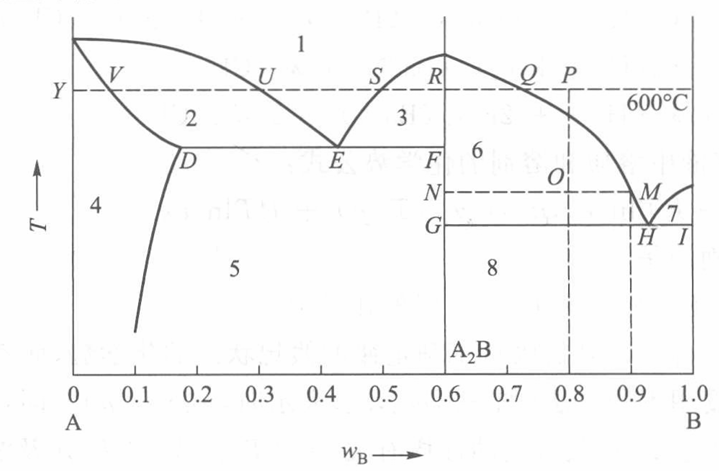
\includegraphics[width=0.52\textwidth]{./Figure/P_2012_5}

\end{figure}

\vspace{0.5cm}
\noindent\textbf{六、计算题(15 pts.)}

$25^\circ\mathrm{C}$时,正辛烷$\ce{C8H18(g)}$的标准燃烧焓是$-5\ 512.4\ \mathrm{kJ\cdot mol^{-1}}$,二氧化碳和液态水的标准生成焓分别为$-393.5\ \mathrm{kJ\cdot mol^{-1}}$和$-285.8\ \mathrm{kJ\cdot mol^{-1}}$,正辛烷、$\ce{H2(g)}$和石墨的标准摩尔熵分别为$463.7\ \mathrm{J\cdot K^{-1}\cdot mol^{-1}}$、$130.6\ \mathrm{J\cdot K^{-1}\cdot mol^{-1}}$及$5.694\ \mathrm{J\cdot K^{-1}\cdot mol^{-1}}$。设正辛烷和氢气可视为理想气体。试求:
\begin{enumerate}[label=(\arabic*), itemsep=1ex]
    \item $25^\circ\mathrm{C}$下,正辛烷生成反应的平衡常数$K_p^\ominus$和$K_c^\ominus$；
    \item 增加压力对提高正辛烷的产率是否有利?为什么?
    \item 升高温度对提高产率是否有利?为什么?
    \item 若在$25^\circ\mathrm{C}$及$101.325\ \mathrm{kPa}$下进行反应,平衡混合物中正辛烷的摩尔分数能否达到$0.1$?若希望正辛烷的摩尔分数在平衡混合物中达$0.5$,在$25^\circ\mathrm{C}$时,需要多大的压力才行?
\end{enumerate}

\vspace{0.5cm}
\noindent\textbf{七、计算题(15 pts.)}

双环戊烯单分子气相热分解反应,$210^\circ\mathrm{C}$时反应的$k_1=2.05\times10^{-4}\ \mathrm{s^{-1}}$,$272^\circ\mathrm{C}$时$k_2=1.86\times10^{-2}\ \mathrm{s^{-1}}$。试求:
\begin{enumerate}[label=(\arabic*), itemsep=1ex]
    \item $210^\circ\mathrm{C}$时反应的半衰期；
    \item 反应的活化能$E_\mathrm{a}$；
    \item 反应在$227^\circ\mathrm{C}$时的活化焓和活化熵。
\end{enumerate}

\vspace{0.5cm}
\noindent\textbf{八、计算题(20 pts.)}

电池$\ce{Zn(S) | ZnCl2(0.05mol\cdot kg^{-1}) | AgCl(s) | Ag(s)}$的电动势与温度的关系为$E/\mathrm{V}=1.015-4.92\times10^{-4}(T/\mathrm{K}-298)$。
\begin{enumerate}[label=(\arabic*), itemsep=1ex]
    \item 写出电池反应；
    \item 计算$298\ \mathrm{K}$时上述电池可逆输出$2F$电荷量时,电池反应的$\Delta_\mathrm{r}G_\mathrm{m}$,$\Delta_\mathrm{r}S_\mathrm{m}$,$\Delta_\mathrm{r}H_\mathrm{m}$,$\Delta_\mathrm{r}U_\mathrm{m}$,$\Delta_\mathrm{r}A_\mathrm{m}$
    
    以及该电池的热效应；
    \item 若将该电池短路,上述各热力学值为多少?
    \item 若该电池以$0.8\ \mathrm{V}$工作电压放电,上述各值又为多少?
\end{enumerate}